         \chapter{Die Hidrosfeer}\fancyfoot[LO,RE]{Chemistry: Chemical systems}
%     \setcounter{figure}{1}
%     \setcounter{subfigure}{1}

    \section{Inleiding}
            \nopagebreak
%             \label{m38138*cid2} $ \hspace{-5pt}\begin{array}{cccccccccccc}   \end{array} $ \hspace{2 pt}\raisebox{-0.2em}{
\includegraphics[height=1em]{../icons/www.pdf}} {(section shortcode: P10107 )}  
\begin{minipage}{.7\textwidth}
So ver ons weet is die Aarde waarop ons bly die enigste planeet wat lewe kan onderhou. Die aarde is, onder andere, die regte afstand van die son af weg sodat die temperatuur van so  'n aard is dat dit lewe kan onderhou. So ook het die aarde se atmosfeer net die regte kombinasie en tipe gasse in die regte verhoudings sodat daar lewe kan wees. Wat ons planeet nog meer uniek maak is die feit dat ons \textbf{water} op die oppervlak het, trouens dit is hoekom die Aarde die Blou Planeet genoem word – die grootste deel van die aarde is onder water. Hierdie watermassas word saamgestel uit \textsl{varswater} in riviere en mere, \textsl{soutwater} in die oseane en riviermondings, \textsl{grondwater} en \textsl{waterdamp}. As  'n geheel staan hierdie watermassas bekend as die \textbf{hidrosfeer}.
\end{minipage}
\begin{minipage}{.3\textwidth}
\begin{center}
 \includegraphics[width=0.6\textwidth]{photos/earth_space_nasa-flickr.jpg}\\
\textsl{Photo by NASA on flickr}
\end{center}

\end{minipage}

\Note{Die totale massa van die hidrosfeer is ongeveer $1,4~{\times}{10}^{18} ~~ \text{ton}$! (Die volume van 1 ton water is ongeveer 1 kubieke meter – dit is ongeveer 900 A4 handboeke!)}

\section{Wisselwerking van die hidrosfeer}
            \nopagebreak

Die hidrosfeer is nie  'n geïsoleerde sisteem nie, dit funksioneer op  'n gereelde basis in wisselwerking met ander globale sisteme insluitend die \textsl{atmosfeer}, \textsl{litosfeer} en \textsl{biosfeer}. As  'n geheel gesien word hierdie interaksie gewoonlik die waterkringloop genoem.

\mindsetvid{the water cycle}{VPbzy}

      \label{m38138*id334463}\begin{itemize}[noitemsep]
            \label{m38138*uid1}\item \textsl{Atmosfeer}
Wanneer water verhit word (bv. deur die energie van die son), verdamp dit en vorm waterdamp. Wanneer waterdamp afkoel, vind kondensasie plaas en vorm dit vloeistof wat uiteindelik weer in die vorm van neerslag (bv. re\"{e}n of sneeu) na die oppervlak terugkeer. Hierdie waterkringloop wat deur die atmosfeer beweeg en die energie verandering wat daarmee gepaard gaan beïnvloed regstreeks die weerpatrone van die aarde.
\label{m38138*uid2}\item \textsl{Litosfeer} \\
\begin{minipage}{.6\textwidth}
In die litosfeer (die oseaan en die kontinentale kors op die Aarde se oppervlak) is water  'n belangrike verweringsagent. Dit beteken dat water help om rotse af te breek na rotsfragmente en uiteindelik na grond. Hierdie fragmente word dikwels deur water weggevoer en op ander plekke gedeponeer. Hierdie twee prosesse (verwering en die vervoer van fragmente) word saam \textbf{erosie} genoem. Erosie help om die aarde se oppervlak te vorm.  'n Voorbeeld hiervan is duidelik in riviere: Ho\"{e}r op in die rivier verweer rotse en die sediment word deur die rivier afgespoel en op die wye vloedvlaktes laer af gedeponeer. Op  'n groter skaal het die beweging van water riviervallei uit berge gevorm en is die grotte en kranse langs die rotsagtige kuslyne almal deur verwering en erosie deur water gevorm.
\end{minipage}
\begin{minipage}{.4\textwidth}
 \begin{center}
  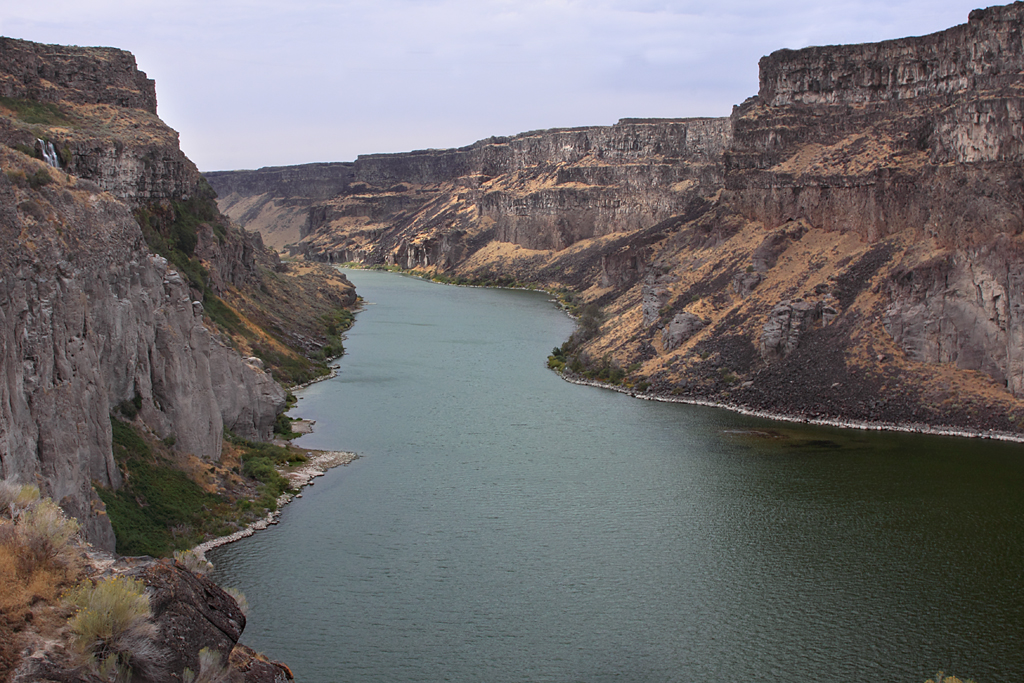
\includegraphics[width=.6\textwidth]{photos/AlanVernon.jpg}\\
\textsl{photo by AlanVernon on flickr}
 \end{center}
\end{minipage}
\label{m38138*uid3}\item \textsl{Biosfeer}
In die biosfeer neem plante water deur hul wortels op en vervoer dit deur hul vaskul\^{e}re stelsels na die stingels en blare. Water is nodig vir \textsl{fotosintese}, die proses waardeur plante voedsel produseer. Deur middel van transpirasie (waar water van die blaaroppervlak verdamp) beweeg water weer in die atmosfeer in.
\end{itemize}


\section{Ondersoek die Hidrosfeer}
            \nopagebreak

Die groot hoeveelheid water op die aarde is  'n unieke verskynsel. Omtrent 71\% van die aarde is bedek met water waarvan 97\% soutwater in die oseane is, 2.2\% as vastestowwe in yslae voorkom en die res (minder as 1\%) varswater is. Ten spyte van die groot hoeveelheid water op die planeet is daar egter slegs  'n klein hoeveelheid wat beskikbaar en geskik is vir menslike verbruik (soos drinkwater). 
Ons het in Reaksies in wateroplossings gekyk na van die reaksies wat in wateroplossings plaasvind en kennis gemaak met die chemiese samestelling van water. In hierdie afdeling gaan ons die hidrosfeer in detail ondersoek sodat ons kan verstaan watter komplekse, maar beeldskone, deel van die wêreld dit beslaan. Nadat jy die volgende ondersoek gedoen het, behoort jy al klaar  'n idee te kry waarom dit belangrik is om bewus te wees van die chemiese samestelling van water.
\label{m38138*secfhsst!!!underscore!!!id86}
            \begin{Investigation}{Ondersoek die hidrosfeer }
            \nopagebreak 
\begin{minipage}{.5\textwidth}
            \label{m38138*uid4}
Vir doeleindes van die oefening kan jy enige deel van die hidrosfeer kies wat jy wil ondersoek. Jy kan  'n rotspoel,  'n meer,  'n rivier,  'n vleiland of selfs  'n klein dammetjie gebruik. Die riglyne hieronder is gebaseer op  'n ondersoek in  'n rivier, maar dit is moontlik om soortgelyke vrae te gebruik en soortgelyke data te versamel in die area wat jy gekies het. Neem in ag hoe toeganklik (kan jy maklik daar kom?)  'n area is wanneer jy die ligging vir jou studie kies asook watter moontlike probleme daar mag wees (soos bv. getye of re\"{e}n).\par
\label{m38138*uid5}
Jou onderwyser sal die toerusting verskaf wat jy nodig het om die volgende data te versamel. Jy moet ten minste een ligging h\^{e} om data te versamel, maar indien jy resultate sou wou vergelyk kan jy nog een kies. So  'n vergelykende studie werk die beste in  'n rivier waar jy langs die lengte van die rivier verskillende areas kan kies. \par
\end{minipage}
\begin{minipage}{.5\textwidth}
\begin{center}
 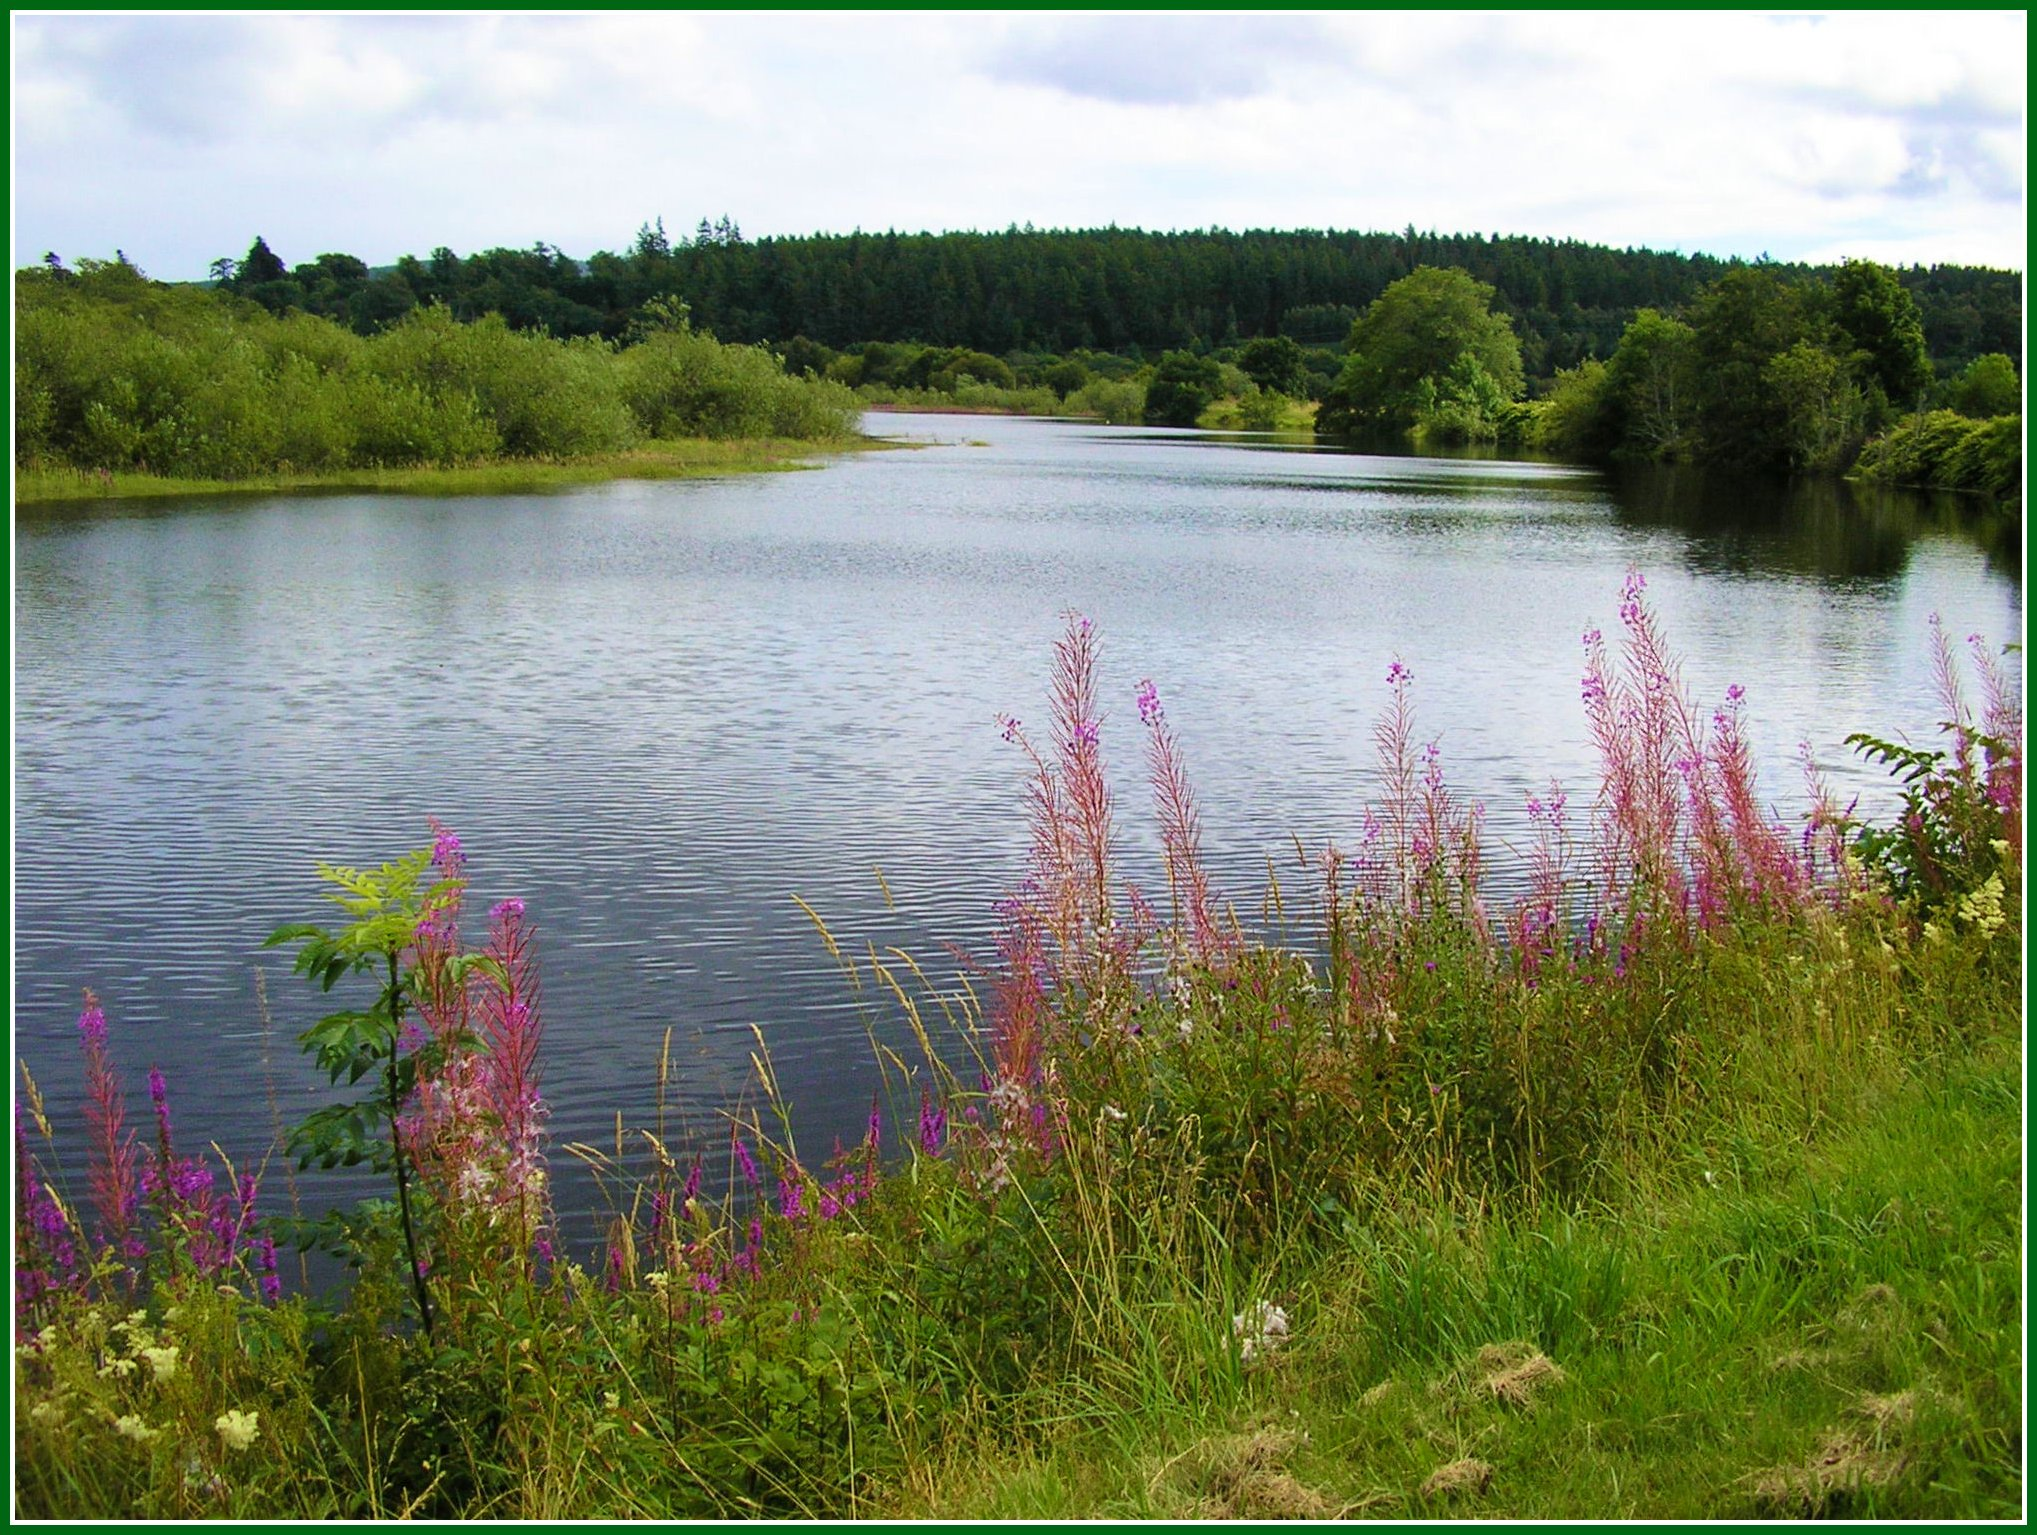
\includegraphics[width=.8\textwidth]{photos/DuncanBrown(Cradlehall).jpg} \\
\textsl{Photo by Duncan Brown (Cradlehall) on flickr}
\end{center}
\end{minipage}
\label{m38138*id334646}\begin{enumerate}[noitemsep, label=\textbf{\arabic*}. ] 
            \label{m38138*uid6}\item \textsl{Chemiese data}
Meet en rekordeer data soos temperatuur, pH, geleidingsvermoë en die opgeloste suurstof by elke ligging. Alhoewel jy moontlik nie op die oomblik verstaan wat hierdie metings beteken nie, sal dit later vir jou duidelik word.
\label{m38138*uid7}\item \textsl{Hidrologiese data}
Meet die water snelheid van die rivier en observeer hoe die volume van die water varieer soos jy in die lengte van die rivier af beweeg. Jy kan ook  'n watermonster in  'n helder plastiekbottel versamel en kyk of die water helder is en of dit deeltjies in het.
\label{m38138*uid8}\item \textsl{Biologiese data}
Watter soorte diere en plante vind jy in of naby hierdie deel van die hidrosfeer? Het hulle spesiaal aangepas by hul omgewing?
\end{enumerate}

Teken jou data in 'n tabel, soos die een hieronder getoon, aan:
% Record your data in a table like the one shown below:
    % \textbf{m38138*id334712}\par
          \begin{table}[H]
    % \begin{table}[H]
    % \\ 'id3029941' '1'
        \begin{center}
      \label{m38138*id334712}
    \noindent
      \begin{tabular}{|l|l|l|l|}\hline
         &
        \textbf{Ligging 1} &
        \textbf{Ligging 2} &
        \textbf{Ligging 3} \\ \hline
        \textbf{Temperatuur} &
         &
         &
       \\ \hline
        \textbf{pH} &
         &
         &
      \\ \hline
        \textbf{Geleidingsvermo\"{e}} &
         &
         &
       \\ \hline
        \textbf{Opgeloste suurstof} &
         &
         &
        \\ \hline
        \textbf{Diere} &
         &
         &
        \\ \hline
        \textbf{Plante} &
         &
         &
        \\ \hline
    \end{tabular}
      \end{center}
\end{table}
    \par
  \label{m38138*uid9}\item \textbf{Interpreteer die data}
Sodra jy jou data versamel en opgeteken het, oorweeg die volgende vrae:
\label{m38138*id334958}\begin{itemize}[noitemsep]
            \label{m38138*uid10}\item Hoe verskil die data van die verskillende liggings?
\label{m38138*uid11}\item Kan jy die verskille verduidelik? 
\label{m38138*uid12}\item Watter effek het die \textsl{pH}, \textsl{temperatuur} en \textsl{opgeloste suurstof} op die diere en plante wat in die hidrosfeer bly?
\label{m38138*uid13}\item Water is selde “suiwer”. Daar is gewoonlik verskeie stowwe in opgelos (bv. ${\text{Mg}}^{2+}$, ${\text{Ca}}^{2+}$ en $\text{NO}_{3}^{-}$ ione) of in suspensie (bv. gronddeeltjies, oorblyfsels). Waar kom hierdie stowwe van daan?
\label{m38138*uid14}\item Is daar enige bewyse van menslike bedrywighede naby hierdie deel van die hidrosfeer? Watter effek kan dit op die hidrosfeer h\^{e}?
\end{itemize}
\end{Investigation}


\section{Die belangrikheid van die Hidrosfeer}
            \nopagebreak

      \label{m38138*id335077}Ons beskou maklik die bestaan van die hidrosfeer as vanselfsprekend, maar hoeveel keer staan ons regtig stil en oordink die rol wat ons planeet speel om ons aan die lewe te hou? Hieronder is  'n paar belangrike funksies van die hidrosfeer:
      \label{m38138*id335082}\begin{itemize}[noitemsep]
            \label{m38138*uid15}\item \textsl{Water is deel van lewende selle}
Elke sel is  'n lewende organisme wat uit omtrent 75\% water bestaan wat die sel normaal laat funksioneer. Trouens, die meeste chemiese reaksies wat in die lewe plaasvind gebeur met stowwe wat in water opgelos is. Sonder water kon selle nie normaal funksioneer nie en sou daar nie lewe wees nie.
\label{m38138*uid16}\item \textsl{Water voorsien habitat}
Die hidrosfeer is  'n belangrike plek vir plante en diere om te bly. Baie gasse (bv. ${\text{CO}}_{2}$, ${\text{O}}_{2}$), voedingstowwe bv. nitraat ($\text{NO}_{3}^{-}$), nitrite ($\text{NO}_{2}^{-}$) en ammonium ($\text{NH}_{4}^{+}$) ione, sowel as ander ione (bv. ${\text{Mg}}^{2+}$ en ${\text{Ca}}^{2+}$) word opgelos in water. Die teenwoordigheid van hierdie stowwe is kritiek tot die bestaan van lewe in water.
\label{m38138*uid17}\item \textsl{Regulering van klimaat}
Een van die unieke karaktereienskappe van water is die \textsl{ho\"{e} spesifieke warmtekapasiteit}. Dit beteken dat dit lank neem vir water om te verhit en ook lank neem om af te koel. Dit speel  'n belangrike rol in die regulering van die aarde se temperatuur om te verseker dat die temperatuur binne die aanvaarbare grense bly vir lewe om te bestaan. \textsl{Seestrome} help ook met die verspreiding van hitte.
\label{m38138*uid18}\item \textsl{Menslike behoeftes}
Mense gebruik water op verskillende maniere. Uiteraard is drinkwater baie belangrik, maar die huishoudelike gebruik van water (bv. vir was en skoonmaak) en die gebruik daarvan in die industrie\"{e} speel ook  'n rol. Water kan ook vir die opwek van elektrisiteit gebruik word deur hidrokrag.
\end{itemize}
Hierdie is maar  'n paar funksies van water op ons planeet. Baie van die ander funksies vind ons in die chemiese samestelling van water en die wyse waarop stowwe in water kan oplos.


\section{Bedreigings vir die hidrosfeer}
            \nopagebreak

Jy behoort teen hierdie tyd te besef dat die hidrosfeer  'n baie belangrike rol speel om lewe op Aarde te onderhou en dat die unieke samestelling van water verskillende belangrike chemiese prosesse laat gebeur wat andersins nie moontlik sou wees nie. Daar is ongelukkig verskeie faktore wat die bestaan van ons hidrosfeer bedreig. Ongelukkig is die meeste van hierdie bedreigings as gevolg van menslike bedrywighede. Ons gaan op twee kwelpunte fokus: \textbf{besoedeling} en die \textbf{oormatige gebruik} of misbruik van die hidrosfeer. Ons gaan ook kyk na moontlike oplossings vir hierdie probleme.

\mindsetvid{water in south africa}{VPcbf} \\

      \label{m38138*id342223}\begin{enumerate}[noitemsep, label=\textbf{\arabic*}. ] 
            \label{m38138*uid91}\item \textbf{Besoedeling}\newline
Besoedeling van die hidrosfeer is  'n reuse probleem. As ons aan besoedeling dink, dink ons gewoonlik net aan die invloed van goed soos plastiek, bottels, olie ensovoorts, maar enige chemikalie wat in die verkeerde verhouding in die hidrosfeer teenwoordig is, is  'n besoedelende stof. Diere en plante wat in die aarde se watermassas bly is spesiaal aangepas om te oorleef binne sekere grense van normale toestande. Wanneer hierdie toestande verander (deur byvoorbeeld besoedeling) kan hierdie organismes nie oorleef nie. Besoedeling affekteer dus die hele akwatiese ekosisteem Die mees algemene vorm van besoedeling in die hidrosfeer is afvalstowwe van mense en industrie\"{e}, nutriënt besoedeling (bv. die afloop van bemesting wat eutrofikasie (waar  'n oormaat nutriënte lei tot oormatige plantegroei) veroorsaak) en toksiese spoorelemente soos aluminium, kwik en koper om maar net  'n paar te noem. Die meeste van hierdie elemente kom van myne of mynbou industrieë.
\label{m38138*uid87}\item \textbf{Oormatige gebruik van water}\newline
Ons het vroe\"{e}r verwys na hoe slegs  'n klein persentasie van die hidrosfeer se water beskikbaar is as varswater. Ten spyte van hierdie feit gebruik die mens al meer water, tot so  'n mate dat die waterverbruik vinnig die hoeveelheid water wat beskikbaar is bereik. Hierdie is  'n ernstige probleem, veral in lande soos Suid-Afrika wat van nature droog is en waar die waterbronne beperk is. Daar word beraam dat die watervoorsiening in Suid-Afrika tussen 2020 en 2040 nie meer die groeiende behoefte vir water in die land sal kan ondersteun nie. Dit het grootliks te make met bevolkingsgroei, maar ook met die groeiende behoefte van industrieë wat daagliks vergroot en ontwikkel. Dit behoort ons koud te laat. Verbeel jou  'n dag sonder water...dis moeilik, nê? Water is so  'n integrale deel van ons lewens dat ons nie eintlik bewus is van hoe  'n groot rol dit in ons daaglikse lewens speel nie.
\end{enumerate}
\label{m38138*secfhsst!!!underscore!!!id1046}
            \begin{groupdiscussion}{ Kreatiewe waterbesparing
}
            \nopagebreak

\label{m38138*uid289435}Namate die bevolking groei, groei die vraag na water en word die druk op ons watervoorsieningsbronne al hoër. Alhoewel baie mense die bou van damme voorhou as  'n oplossing vir hierdie tekort is daar bewyse dat damme slegs  'n tydelike oplossing is. Baie keer rig hierdie oplossing op die ou einde groter ekologiese skade aan as wat dit  'n oplossing bied. Die enigste volhoubare oplossing is om die vraag na water te verminder totdat die waterbronne die vraag kan bevredig. Die groot vraag is dus hoe om dit te doen?\\
\label{m38138*uid5630}\textbf{Bespreking:}
\begin{minipage}{.6\textwidth}
 Verdeel die klas in groepe van ongeveer vyf. Elke groep verteenwoordig  'n ander sektor van die samelewing. Julle onderwyser sal die verskillende groepe vir julle aanwys: Boerdery, Industrie, Stadsbestuur, Waterbesparing, Toerisme of Burgerlike samelewing (julle verteenwoordig met ander woorde die gewone burgers, die sogenaamde “man op die straat”) Bespreek die volgende vrae in jul groepe met verwysing na die sektor wat julle verteenwoordig: (Onthou om notas te neem tydens julle bespreking. Nomineer  'n woordvoerder om namens julle aan die res van die klas terugvoer te gee.)
\end{minipage}
\begin{minipage}{.4\textwidth}
 \begin{center}
  \includegraphics[width=.6\textwidth]{photos/karoo_flowcomm.jpg} \\
\textsl{Photo by flowcomm on flickr}
 \end{center}

\end{minipage}
\label{m38138*id342317}\begin{itemize}[noitemsep]
            \label{m38138*uid88}\item Watter stappe moet jou groep neem om water te bespaar?
\label{m38138*uid89}\item Waarom word hierdie stappe nie tans geneem nie?
\label{m38138*uid90}\item Watter aansporingsbonusse kan gebied word om die groep te oortuig om water meer effektief te bespaar?
\end{itemize}


\end{groupdiscussion}
\par 
\label{m38138*id0123}
            \begin{Investigation}{Die bou van damme}
            \nopagebreak

\label{m38138*id0128031}In die vorige bespreking het ons verwys daarna dat daar bewyse is dat die bou van damme slegs  'n tydelike oplossing is vir die waterkrisis. Hierdie ondersoek gaan kyk na waarom damme potensieel  'n slegte oplossing vir die probleem is. \\
\label{m38138*id473692}Kies  'n dam wat in jou area, of  'n area naby jou, gebou is. Kyk watter riviere in jou area is. Probeer om die volgende vrae te antwoord: \\
\begin{minipage}{.7\textwidth}
\label{m38138*id774}\begin{itemize}[noitemsep]
            \label{m38138*id034582}\item Indien moontlik gesels met mense wat al lank in die area bly en probeer hulle opinie kry oor hoe die lewe verander het sedert die dam gebou is. As daar nie sulke mense in die area is nie, probeer relevante literatuur oor die area opspoor.
\label{m38138*id08323}\item Probeer uitvind of  'n omgewingsimpakstudie (dit is wanneer mense die omgewing bestudeer om te kyk watter moontlike effek  'n voorgestelde projek op die omgewing kan hê) gedoen is voor die dam gebou is. Waarom dink jy is dit belangrik?
\label{m38138*id0832346}\item 
Kyk na veranderinge in die ekologie. Wat was die ekologie van die rivier voor die dam gebou is? Wat is die bestaande ekologie? Dink jy die verandering was goed of sleg? Jy kan moontlik onderhoude voer met mense wat lank voor die dam gebou is in die area gebly het. 
\end{itemize}
        \par 
\end{minipage}
\begin{minipage}{.3\textwidth}
 \begin{center}
  \includegraphics[height=.8\textwidth]{photos/Redeo.jpg} \\
\textsl{Photo by Redeo on flickr}
 \end{center}

\end{minipage}
\label{m38138*id08322432}
Skryf  'n verslag of doen  'n aanbieding in die klas oor jou bevindinge. Evalueer jou bevindinge krities en maak jou eie gevolgtrekkings oor of die bou van damme slegs  'n kort termyn oplossing vir  'n lang termyn probleem is.
\end{Investigation}
      \label{m38138*id342412}Dit is belangrik dat jy verstaan dat daar  'n fyn balans is tussen die bestaan van ons hidrosfeer en ander sisteme. Wanneer hierdie balans versteur word kan dit ernstige gevolge inhou vir lewe op hierdie planeet.
\label{m38138*secfhsst!!!underscore!!!id1065}
            \begin{project}{Skool Aksie Projek
      }
            \nopagebreak
 'n Skool kan baie doen om water binne skoolverband te bespaar. Bespreek as  'n klas watter stappe julle moet neem om mense meer bewus te maak van hoe belangrik dit is om water te bespaar. Besin ook oor maniere waarop julle skool water kan bespaar. Kyk of julle van hierdie idees prakties kan toepas en kyk of dit regtig water bespaar. Stap tydens pouse rond en maak  'n lys van al die plekke by die skool waar water gemors word.
\end{project}

\section{Hoe suiwer is ons water?}
            \nopagebreak

As jy  'n glas water drink, drink jy nie net water nie, maar ook al die ander stowwe wat daarin opgelos is. Van hierdie stowwe het oorgebly van die proses waardeur water veilig gemaak word vir die mens om te drink en ander kom van die omgewing. Selfs al drink jy water uit  'n bergstroom (wat baie maal as suiwer beskou word en gebotteleer word vir mense om te drink) is daar nogsteeds onsuiwerhede in die water. Waterbesoedeling verhoog die hoeveelheid onsuiwerhede in die water en maak dit soms onveilig om te drink. In hierdie afdeling kyk ons na van die stowwe wat water onsuiwer maak en ons kyk hoe ons suiwer water kan maak. Ons gaan ook kyk na die pH van water.
\par 
\label{m38138*id08324}
In hoofstuk~\ref{chap:rxnsaq} het ons gekyk hoe verbindings in water opgelos kan word. Die meeste van hierdie verbindings (bv. ${\text{Na}}^{+}$, ${\text{Cl}}^{-}$, ${\text{Ca}}^{2+}$, ${\text{Mg}}^{2+}$, ens.) wat natuurlik in die water teenwoordig is, is veilig vir die mens om in klein hoeveelhede in te neem. Wanneer hierdie ione bo wat beskou word as veilige vlakke styg, is die water besoedel.
\par 
\label{m38138*id08322346}Jy het dalk al opgemerk dat water wat jy uit die kraan tap soms  'n skerp reuk het. Jy sal dieselfde reuk by die swembad kry as gevolg van die chloor in die water. Chloor is die mees algemene verbinding wat by water gegooi word om dit vir die mens veilig te maak. Chloor help om bakterie\"{e} en ander biologiese smetstowwe uit die water te haal. Ander metodes om water te suiwer sluit filtrasie (om water deur  'n baie fyn maas te gooi) en flokkulasie ( 'n proses waardeur chemikalieë by water gevoeg word om klein deeltjies te verwyder) in.  
\par 
\label{m38138*id0832}
Die pH van water is ook belangrik. Water wat te basies (pH hoër as 7) of te suur (pH laer as 7) is, kan probleme inhou vir menslike verbruik. As jy al agtergekom het dat jou oë rooi en jou vel krapperig is nadat jy geswem het, was die pH in die swembad waarskynlik te basies of te suur. Dit wys jou hoe sensitief ons is vir enige veranderinge in ons omgewing. Die pH van water hang af van die ione wat daarin opgelos is. As jy chloor by water gooi, verlaag dit gewoonlik die pH. Jy sal meer leer van pH in graad 11.
\label{m38138*id08321}
            \begin{g_experiment}{Die suiwerheid van water/Hoe suiwer is water.}
            \nopagebreak
            \label{m38138*id08341}\noindent{}\textbf{Doel:}\newline
Om die suiwerheid en pH van water te toets.
\\
\label{m38138*id083244}\noindent{}\textbf{Apparaat:}\\
\begin{minipage}{.5\textwidth}
pH toetstrokies (jy kan dit by dierewinkels kry, hulle gebruik dit om die pH van vistenke te meet), mikroskoop (of vergrootglas), filtreerpapier, tregter, silwernitraat, gekonsentreerde soutsuur, bariumchloried, suur, chloorwater ( 'n oplossing van chloor in water), koolstoftetrachloried,  'n paar toetsbuise of –bekers, watermonsters van verskillende bronne (bv.  'n rivier,  'n dam, die see, kraanwater ens.)
\end{minipage}
\begin{minipage}{.5\textwidth}
%  \begin{figure}

\begin{center}
\scalebox{0.5} % Change this value to rescale the drawing.
{
\begin{pspicture}(-5,-5)(5,5)
\psset{unit=1cm}
\newpsstyle{white} {linestyle=solid,linewidth=.1,fillstyle=solid,fillcolor=white}
\rput(-4,0){\pstTubeEssais[niveauLiquide1=40,aspectLiquide1=white]}
\psline[linewidth=0.04]{->}(-3.8,-1)(-3,-1)
\uput[r](-3,-1){\large{sea}}
\rput(0,0){\pstTubeEssais[niveauLiquide1=40,aspectLiquide1=white]}
\psline[linewidth=0.04]{->}(0.2,-1)(1,-1)
\uput[r](1,-1){\large{river}}
\rput(4,0){\pstTubeEssais[niveauLiquide1=40,aspectLiquide1=white]}
\psline[linewidth=0.04]{->}(4.2,-1)(5,-1)
\uput[r](5,-1){\large{rain}}
\rput(8,0){\pstTubeEssais[niveauLiquide1=40,aspectLiquide1=white]}
\psline[linewidth=0.04]{->}(8.2,-1)(9,-1)
\uput[r](9,-1){\large{tap}}
\end{pspicture}
}
\end{center}
% \end{figure}
\end{minipage}
\\
\label{m38138*id438234}\noindent{}\textbf{Metode:}
\label{m38138*id827732}\begin{enumerate}[noitemsep, label=\textbf{\arabic*}. ] 
            \item Kyk na elke watermonster en skryf neer of die water helder of troebel is.
\item Bestudeer elke watermonster onder  'n mikroskoop en skryf neer wat jy sien.
\item Toets die pH van elke watermonster.
\item Gooi van die water van elke monster deur die filtreerpapier.
\item Verwys na Toets vir algemene anione in oplossings vir die besonderhede van die algemene anioon toets. Toets vir chloor, sulfate, karbonate, bromiede en jodiede in elke watermonster.\end{enumerate}
\\
\label{m38138*id63284}\noindent{}\textbf{Resultate:}\\
Skryf neer wat jy gesien het toe jy net na die watermonsters gekyk het. Skryf neer wat jy gesien het toe jy onder  'n mikroskoop na die watermonsters gekyk het. Was daar enige opgeloste deeltjies? Was daar iets anders in die water? Was daar  'n verskil tussen wat jy gesien het toe jy net na die water gekyk het en toe jy na dit onder die mikroskoop gekyk het? Skryf die pH van elke watermonster neer. Kyk na elke monster se filtreerpapier. Is daar sand of ander deeltjies op die filtreerpapier? Watter anione het jy in elke monster gekry?
\\
\label{m38138*id3429827}\noindent{}\textbf{Bespreking:}\\
Skryf  'n verslag oor jou waarnemings. Maak gevolgtrekkings oor die suiwerheid van die water en hoe jy kan sê of die water suiwer is al dan nie.
\\  
\label{m38138*id68921}\noindent{}\textbf{Gevolgtrekking:}\\
Jy moes gesien het dat water nie suiwer is nie, maar eerder verskillende stowwe het wat daarin opgelos is.
\\
\end{g_experiment}
\label{m38138*id672214}
            \begin{project}{Watersuiwering}
            \nopagebreak
\label{m38138*id97324}
Berei  'n aanbieding voor oor hoe water gesuiwer word. Jy het  'n keuse tussen  'n plakkaat,  'n aanbieding of  'n geskrewe verslag. Jy moet die volgende aandag gee aan:
\label{m38138*id097324}\begin{itemize}[noitemsep]
            \item Water om te drink (drinkbare water)
\item Gedistilleerde water en die gebruik daarvan
\item Deioniseerde water en die gebruik daarvan
\item Watter metodes gebruik word om water voor te berei vir die verskillende gebruike daarvan.
\item Watter regulasies heers vir drinkwater
\item Waarom water gesuiwer moet word.
\item Hoe veilig hierdie suiweringsmetodes is.
\end{itemize}
\par 
\end{project}


\summary{VPfbj}
            \nopagebreak

\begin{itemize}[noitemsep]
\item Die \textbf{hidrosfeer} sluit al die water wat op die Aarde is in. Bronne van water sluit varswater (bv. rivere en mere), soutwater (bv. oseane), grondwater (bv. boorgate) en waterdamp in. Ys (bv. gletsers)  is ook deel van die hidrosfeer.
\label{m38138*uid93}\item Die hidrosfeer is in wisselwerking met die ander globale sisteme insluitende die atmosfeer, litosfeer en biosfeer.
\label{m38138*uid94}\item Die hidrosfeer het  'n paar belangrike funksies: water is deel van alle lewende selle, dit voorsien  'n habitat vir baie lewende organismes, dit reguleer die klimaat  en word deur mense gebruik  vir huishoudelike, industriële en ander aktiwiteite.
\label{m38138*uid106}\item Ten spyte van die belangrikheid van die hidrosfeer is daar verskeie faktore wat die hidrosfeer bedreig. Oormatige gebruik en besoedeling is ingesluit hierby.
\item Water is nie suiwer nie; daar is baie stowwe daarin opgelos.
\end{itemize}

\begin{eocexercises}{Die hidrosfeer}
            \nopagebreak

\begin{enumerate}[noitemsep, label=\textbf{\arabic*}. ] 
    \item Wat is die hidrosfeer? Hoe is dit in wisselwerking met ander globale sisteme?
    \item Waarom is die hidrosfeer belangrik?
    \item Skryf  'n opstel van een bladsy oor die belangrikheid van water en wat ons kan doen om te verseker dat ons oor 50 jaar nogsteeds drinkbare water het.
\end{enumerate}

% Automatically inserted shortcodes - number to insert 3
\par \practiceinfo
\par \begin{tabular}[h]{cccccc}
% Question 1
(1.)	029a	&
% Question 2
(2.)	029b	&
% Question 3
(3.)	029c	&
\end{tabular}
% Automatically inserted shortcodes - number inserted 3
\end{eocexercises}
